\documentclass[12pt]{article}
\usepackage[utf8]{inputenc}


\usepackage{amsmath}
\usepackage{amssymb}
\usepackage{graphicx}
\usepackage{hyperref}
\usepackage{geometry}
\usepackage{natbib}
\geometry{a4paper, margin=1in}

\title{Sampling From a Discrete Posterior}
\author{Bar Weinstein}
\date{\today}

\begin{document}

\maketitle

\section{Setup}
We have posterior 
\begin{equation}
\label{eq:observed.posterior}
\begin{split}
  p(\eta,\theta,\gamma, A^\ast \vert Y,Z,X,A) 
    \propto
    &\; p(Y \vert Z,A^\ast,X,\eta) p(\eta) 
    \\ & 
  \times p(A \vert A^\ast, X,\gamma) 
   p(\gamma)
    \\ &
   \times p(A^\ast \vert X,\theta) 
   p(\theta),
\end{split}
\end{equation}
where $\eta,\theta,\gamma$ are continuous and $A^\ast$ is
discrete with large dimension $O(N^2)$. 

First approach is to use the cut-posterior 
\begin{equation}
    \label{eq:cut.posterior}
    p_{cut}(\eta,\theta,\gamma,A^\ast \vert Y,Z,X,A) \propto 
    p(\eta \vert Y,Z, A^\ast,X)
    p(\theta,\gamma,A^\ast \vert A, X),
\end{equation}
and sample from it by first sample $\theta,\gamma$, 
then generate $A^\ast$ samples,
and finally sample $\eta$ either via plug-in or multi-stage sampling.
This approach is fine but other than plug-in sampling it takes a while.
We can maybe do better!

Gibbs sampling requires sampling from the full conditional of each.
 Write $O = (Y,Z,X,A)$ for the observed data.
Then the full conditionals are
\begin{equation}
    \label{eq:full.conditionals}
    \begin{split}
     \gamma  &\sim p(\gamma \vert O, \eta,\theta,A^\ast) \propto 
        p(A \vert A^\ast, X,\gamma) p(\gamma) \\
    \theta &\sim p(\theta \vert O, \eta,\gamma,A^\ast) \propto
        p(A^\ast \vert X,\theta) p(\theta) \\
    \eta &\sim p(\eta \vert O, \theta,\gamma,A^\ast) \propto
        p(Y \vert Z,A^\ast,X,\eta) p(\eta) \\
    A^\ast &\sim p(A^\ast \vert O, \eta,\theta,\gamma) \propto
        p(Y \vert Z,A^\ast,X,\eta) p(A \vert A^\ast, X,\gamma) p(A^\ast \vert X,\theta).
    \end{split}
\end{equation}
Sampling $\gamma,\theta,\eta$ is easy, but sampling $A^\ast$ is hard.
The continuous paramteters can be updated with gradient-based methods such as 
MALA or HMC. I'll now present methods for sampling $A^\ast$.

\section{Methods for Discrete Sampling}
Assume that $\mathcal{A}^\ast$ is the space of all possible $A^\ast$.
Naively, we can sample $A*$ by sampling all edges independently. 
However, $A^\ast$ may have global impact on $Y$ so flipping one edge $A^\ast_{ij}$
can impact the the likelihood of $Y_k$ where $k \neq i,j$. 
That will complicate the naive $A^\ast$ updates, e.g., via MH.

Write the log conditional posterior of $A^\ast$ as

\begin{equation}
    \begin{split} 
        \label{eq:conditional.A}
        f(A^\ast) &= \log p(A^\ast \vert O, \eta,\theta,\gamma) 
        \\ &\propto
        \log p(Y \vert Z,A^\ast,X,\eta) + \log p(A \vert A^\ast, X,\gamma) + \log p(A^\ast \vert X,\theta).
    \end{split}
\end{equation}

\begin{enumerate}
    \item \textbf{The Hamming Ball Sampler.}\footnote{ \url{https://www.tandfonline.com/doi/full/10.1080/01621459.2016.1222288}}
            Variant of slice sampling for discrete variables.
            Idea is to have an auxilary variable that constraint the sampling space 
            to a subset of $\mathcal{A}^\ast$. At each iteration we create a ``slice'' 
            (the auxilary variable), sample $A^\ast$ from this slice subset, etc.
            Example of application is to restrict the number of changes of $A^\ast$
            proposal in each iteration and sample from that the Hamming ball of radius $d$.
            Effectively, it is local updates constraints to the number of new changes.
            

    \item \textbf{Informed Proposals}. Basic idea is that in updating $A^\ast$ 
            we propose a new value from a kernel $q(A^{\ast'} \vert A^\ast)$. 
            In fact, we propose each edge seperately so it can be written as 
            $q(A^{\ast'} \vert A^\ast) = \sum_{e} q(A^{\ast'} \vert A^\ast,e)q(e)$, that is, 
            sample edges with $q(e)$ and then ``flip'' the edge with 
            $q(A^{\ast'} \vert A^\ast,e) = I(A^{\ast'}_{ij}=A^\ast_{ij}), \; \forall (i,j)\neq e$.
            Key idea here is what edges $e$ we select to flip. 
            Naive random-walk just select these edges uniformly, but we can do better.
            That is the main idea behind Zanella (2020)\footnote{\url{https://www.tandfonline.com/doi/full/10.1080/01621459.2019.1585255?src=recsys}}
            paper on Informed Proposals.
             
            Assume for now that we only ``flip'' one edge at a time 
            (can be extended for block or sequential updates in each iteration).
            One option is to inform the edge selection by its impact on $f(A^\ast)$ values,
            i.e., on the gradients. Since $A^\ast$ is discrete we don't have gradients.
            As before, write $A^{\ast'}$ as $A^\ast$ where only edge $e$ is ``flipped" ($0\to 1, 1\to 0$).
            Then the score is $d(A^{\ast'},A^\ast) = f(A^{\ast'}) - f(A^\ast)$.
            We can use this score to inform the edge selection by taking proposals 
            $q(A^{\ast'} \vert A^\ast) \propto \exp(d(A^{\ast'},A^\ast)/t)$ where $t$ is a 
            ``temprature'' controlling the locality of the updates. 
            By Zanella (2020), optimal $t$ is $t=2$ in the binary case (so called ``Barker choice").
            The scores are 
            effectively the tempered likelihood ratios.
            However, computing $d(A^{\ast'},A^\ast)$ is expensive since we need to evaluate $f$ twice
            for each possible edges, i.e., at least $O(N^2)$ per iteration. 
            Grathwohl et al. (2021)\footnote{\url{https://proceedings.mlr.press/v139/grathwohl21a.html}}
            proposed to approximate this score by taking 
            a gradient:
            $\widetilde{d}(A^{\ast'},A^\ast) = (A^{\ast'}_e - A^{\ast}_e)\nabla f_{A^\ast_e}(A^\ast_e)$.
            That is, $\widetilde{d}(A^{\ast'},A^\ast) \approx d(A^{\ast'},A^\ast) = f(A^{\ast'}) - f(A^\ast)$,
            where the gradient of $f()$ is taken w.r.t. $A^\ast_e$ as if $A^\ast_e$ is 
            continuous\footnote{It can be performed automatically in torch via \texttt{torch.autograd.grad} or in 
            JAX via \texttt{jax.grad}.}.
            They have some results about this approximation.
            The proposed pseudo-algorithm for $A^\ast$ updates is thus:

            \begin{figure}[!ht]
                \centering
                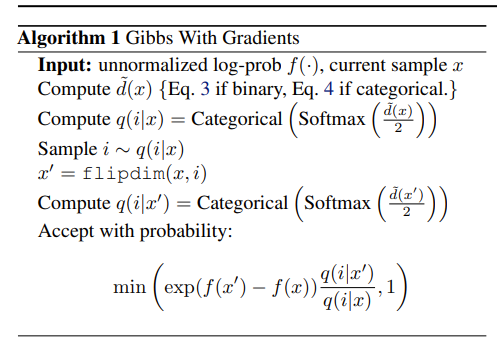
\includegraphics[width=0.6\textwidth]{gwg.png}
                % \caption{Gibbs-With-Gradients.}
            \end{figure}

            Namely, compute scores for edge selection, sample edge with probabilities
            proportional to the scores, flip its edge, compute new scores,
             and accept/reject with MH. 
             This can be extended for either $K$ edges ``flips'' in a block 
             or $K$ sequential flips in each iteration. 
             The cool thing is that don't really have to flip all edges
             in each iteration.

            \textit{Limitations.} To compute the scores $d(A^{\ast'},A^\ast)$ 
            we need to evalutate $f$ twice for each edge flip, i.e., $O(N^2)$ evaluations.
            If $A^\ast$ and $A$ are edge indepdent then, evaluating 
            $\log p(A \vert A^\ast, X,\gamma) + \log p(A^\ast \vert X,\theta)$ is easy
            since each flip only affects one edge. 
            However, the outcome model can possibly depend on global network statistics,
            e.g., eigenvector centrality, so flipping one edge can impact the outcomes of many units!
            That will be computionally expensive to evaluate the scores using the outcomes model.
            One option is to neglect the outcome model in the scores computation, 
            or just use them occasionally (e.g., in every $L$ iterations). 
            That resemble cut-posterior sampling, but not exactly as we sample everything together.
            Need to think if using the gradient with $\widetilde{d}$ will assist even with the outcome model.

            \textit{Multiple updates.} In Grathwohl et al. (2021) approach, in each iteration we ``flip'' one edge.
            It can be updated by sampling $K$ edges from $q(i\vert A^\ast)$ and
            in the accept/reject step write accordingly the new network $A^{\ast'}$ 
            with all the edges flipps, and instead of $q(i \vert A^\ast)$ write
            the product $\prod_k q(i_k \vert A^\ast)$.

            \textbf{Discrete MALA.} Zhang et al. (2022)\footnote{\url{https://proceedings.mlr.press/v162/zhang22t.html}}
            proposed to use \textit{discrete Metropolis-adjusted Langevin algorithm (DMALA)}.
            Their approach builds on Grathwohl et al. (2021). 
            Their idea is that if we can factorize the discrete parameter space 
            $\mathcal{A}^\ast = \prod_e \mathcal{A}^\ast_e = \{0,1\}^D$ with $D=N(N-1)/2$, then we can
            suggest an update for all edges in each iteration, instead of the single
            update in Grathwohl et al. (2021).
            Their methods begins with computing the gradient $\nabla f(A^\ast)$ 
            as approximation for the difference (likelihood ratio) as before. 
            Then we ``flip'' edge $e$ with probability 
            $\frac{\exp\big(\frac{1}{2}\nabla f(A^\ast)_e (A^{\ast'}_e - A^\ast_e) - \frac{1}{2\alpha}\big)}{
                \exp\big(\frac{1}{2}\nabla f(A^\ast)_e (A^{\ast'}_e - A^\ast_e) - \frac{1}{2\alpha}\big) + 1
            } $
            where $\alpha$ is the step size. 
            Namely, we compute once the gradient for all edges, and then propose 
            update (flip) for each edge at once. 
            We accept/reject the update with MH step with the log-probabilities $f$ 
            and the product of selection probabilities.
            \begin{figure}[!ht]
                \centering
                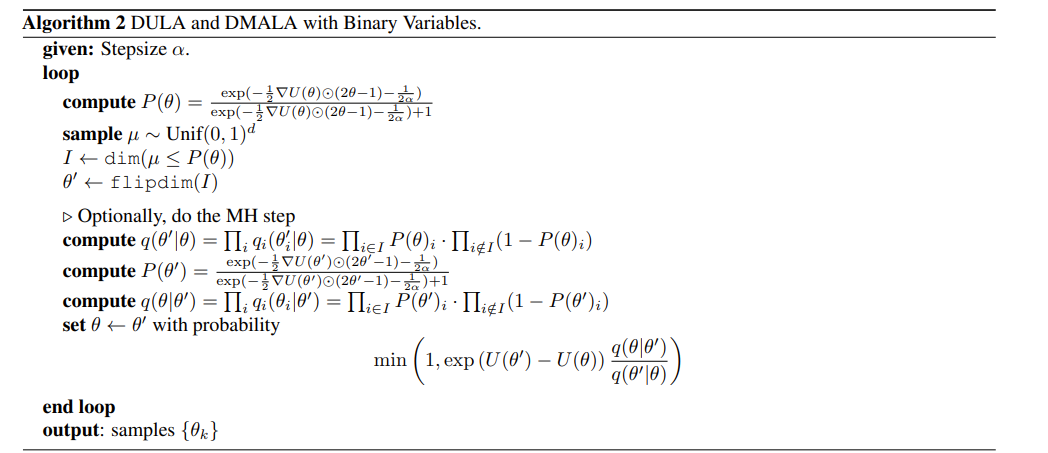
\includegraphics[width=0.99\textwidth]{dmala.png}
                % \caption{DMALA.}
            \end{figure}
            


        \end{enumerate}

\bibliographystyle{plain} % Choose a bibliography style
\bibliography{ref.bib} % Include the references.bib file
    
\end{document}